%%
%% This is file `sample-sigplan.tex',
%% generated with the docstrip utility.
%%
%% The original source files were:
%%
%% samples.dtx  (with options: `sigplan')
%% 
%% IMPORTANT NOTICE:
%% 
%% For the copyright see the source file.
%% 
%% Any modified versions of this file must be renamed
%% with new filenames distinct from sample-sigplan.tex.
%% 
%% For distribution of the original source see the terms
%% for copying and modification in the file samples.dtx.
%% 
%% This generated file may be distributed as long as the
%% original source files, as listed above, are part of the
%% same distribution. (The sources need not necessarily be
%% in the same archive or directory.)
%%
%% The first command in your LaTeX source must be the \documentclass command.

\documentclass[sigconf, nonacm, natbib=false]{acmart}
\usepackage{comment}
\usepackage[english]{babel}
\usepackage[sorting=none]{biblatex}
\usepackage{indentfirst}
\addbibresource{mybib.bib}

%% NOTE that a single column version is required for 
%% submission and peer review. This can be done by changing
%% the \doucmentclass[...]{acmart} in this template to 
%% \documentclass[manuscript,screen,review]{acmart}
%% 
%% To ensure 100% compatibility, please check the white list of
%% approved LaTeX packages to be used with the Master Article Template at
%% https://www.acm.org/publications/taps/whitelist-of-latex-packages 
%% before creating your document. The white list page provides 
%% information on how to submit additional LaTeX packages for 
%% review and adoption.
%% Fonts used in the template cannot be substituted; margin 
%% adjustments are not allowed.
%%
%% \BibTeX command to typeset BibTeX logo in the docs


\begin{comment}
\AtBeginDocument{%
  \providecommand\BibTeX{{%
    \normalfont B\kern-0.5em{\scshape i\kern-0.25em b}\kern-0.8em\TeX}}}

%% Rights management information.  This information is sent to you
%% when you complete the rights form.  These commands have SAMPLE
%% values in them; it is your responsibility as an author to replace
%% the commands and values with those provided to you when you
%% complete the rights form.
\setcopyright{acmcopyright}
\copyrightyear{2018}
\acmYear{2018}
\acmDOI{XXXXXXX.XXXXXXX}

%% These commands are for a PROCEEDINGS abstract or paper.
\acmConference[Conference acronym 'XX]{Make sure to enter the correct
  conference title from your rights confirmation emai}{June 03--05,
  2018}{Woodstock, NY}
%
%  Uncomment \acmBooktitle if th title of the proceedings is different
%  from ``Proceedings of ...''!
%
%\acmBooktitle{Woodstock '18: ACM Symposium on Neural Gaze Detection,
%  June 03--05, 2018, Woodstock, NY} 
\acmPrice{15.00}
\acmISBN{978-1-4503-XXXX-X/18/06}
\end{comment}

%%
%% Submission ID.
%% Use this when submitting an article to a sponsored event. You'll
%% receive a unique submission ID from the organizers
%% of the event, and this ID should be used as the parameter to this command.
%%\acmSubmissionID{123-A56-BU3}

%%
%% The majority of ACM publications use numbered citations and
%% references.  The command \citestyle{authoryear} switches to the
%% "author year" style.
%%
%% If you are preparing content for an event
%% sponsored by ACM SIGGRAPH, you must use the "author year" style of
%% citations and references.
%% Uncommenting
%% the next command will enable that style.
%%\citestyle{acmauthoryear}


%%
%% end of the preamble, start of the body of the document source.
\begin{document}

%%
%% The "title" command has an optional parameter,
%% allowing the author to define a "short title" to be used in page headers.

%%
%% The "author" command and its associated commands are used to define
%% the authors and their affiliations.
%% Of note is the shared affiliation of the first two authors, and the
%% "authornote" and "authornotemark" commands
%% used to denote shared contribution to the research.
\begin{comment}
\author{Ben Trovato}
\authornote{Both authors contributed equally to this research.}
\email{trovato@corporation.com}
\orcid{1234-5678-9012}
\author{G.K.M. Tobin}
\authornotemark[1]
\email{webmaster@marysville-ohio.com}
\affiliation{%
  \institution{Institute for Clarity in Documentation}
  \streetaddress{P.O. Box 1212}
  \city{Dublin}
  \state{Ohio}
  \country{USA}
  \postcode{43017-6221}
}
\end{comment}

\author{Ting-Wei Su}
\affiliation{%
  \institution{Texas A\&M University}
  \city{College Station}
  \country{United States}}
\email{willytwsu@tamu.edu}

\setcopyright{none}
\settopmatter{printacmref=false} % Removes citation information below abstract
\renewcommand\footnotetextcopyrightpermission[1]{} % removes footnote with conference information in first column
%\pagestyle{plain}

\title{Chia Network and Accelerated Plotter}
%%
%% By default, the full list of authors will be used in the page
%% headers. Often, this list is too long, and will overlap
%% other information printed in the page headers. This command allows
%% the author to define a more concise list
%% of authors' names for this purpose.
%%\renewcommand{\shortauthors}{Trovato and Tobin, et al.}

%%
%% The abstract is a short summary of the work to be presented in the
%% article.
\begin{abstract}
  Chia network, a new decentralized network utilizing the proof of space and verified delay function is a recent spotlight in blockchian which came live around May of 2021. The utilization of disk to contribute proof of space is not only innovative but also ecologically friendly. Compared with the most well-known cryptocurrency, bitcoin, the energy consume in chia network is extremely less than the power required during bitcoin mining. 
  

\end{abstract}

%%
%% The code below is generated by the tool at http://dl.acm.org/ccs.cfm.
%% Please copy and paste the code instead of the example below.
%%
\maketitle

\begin{comment}
\begin{CCSXML}
<ccs2012>
 <concept>
  <concept_id>10010520.10010553.10010562</concept_id>
  <concept_desc>Computer systems organization~Embedded systems</concept_desc>
  <concept_significance>500</concept_significance>
 </concept>
 <concept>
  <concept_id>10010520.10010575.10010755</concept_id>
  <concept_desc>Computer systems organization~Redundancy</concept_desc>
  <concept_significance>300</concept_significance>
 </concept>
 <concept>
  <concept_id>10010520.10010553.10010554</concept_id>
  <concept_desc>Computer systems organization~Robotics</concept_desc>
  <concept_significance>100</concept_significance>
 </concept>
 <concept>
  <concept_id>10003033.10003083.10003095</concept_id>
  <concept_desc>Networks~Network reliability</concept_desc>
  <concept_significance>100</concept_significance>
 </concept>
</ccs2012>
\end{CCSXML}

\ccsdesc[500]{Computer systems organization~Embedded systems}
\ccsdesc[300]{Computer systems organization~Redundancy}
\ccsdesc{Computer systems organization~Robotics}
\ccsdesc[100]{Networks~Network reliability}

%%
%% Keywords. The author(s) should pick words that accurately describe
%% the work being presented. Separate the keywords with commas.
\keywords{datasets, neural networks, gaze detection, text tagging}

%% A "teaser" image appears between the author and affiliation
%% information and the body of the document, and typically spans the
%% page.
\begin{teaserfigure}
  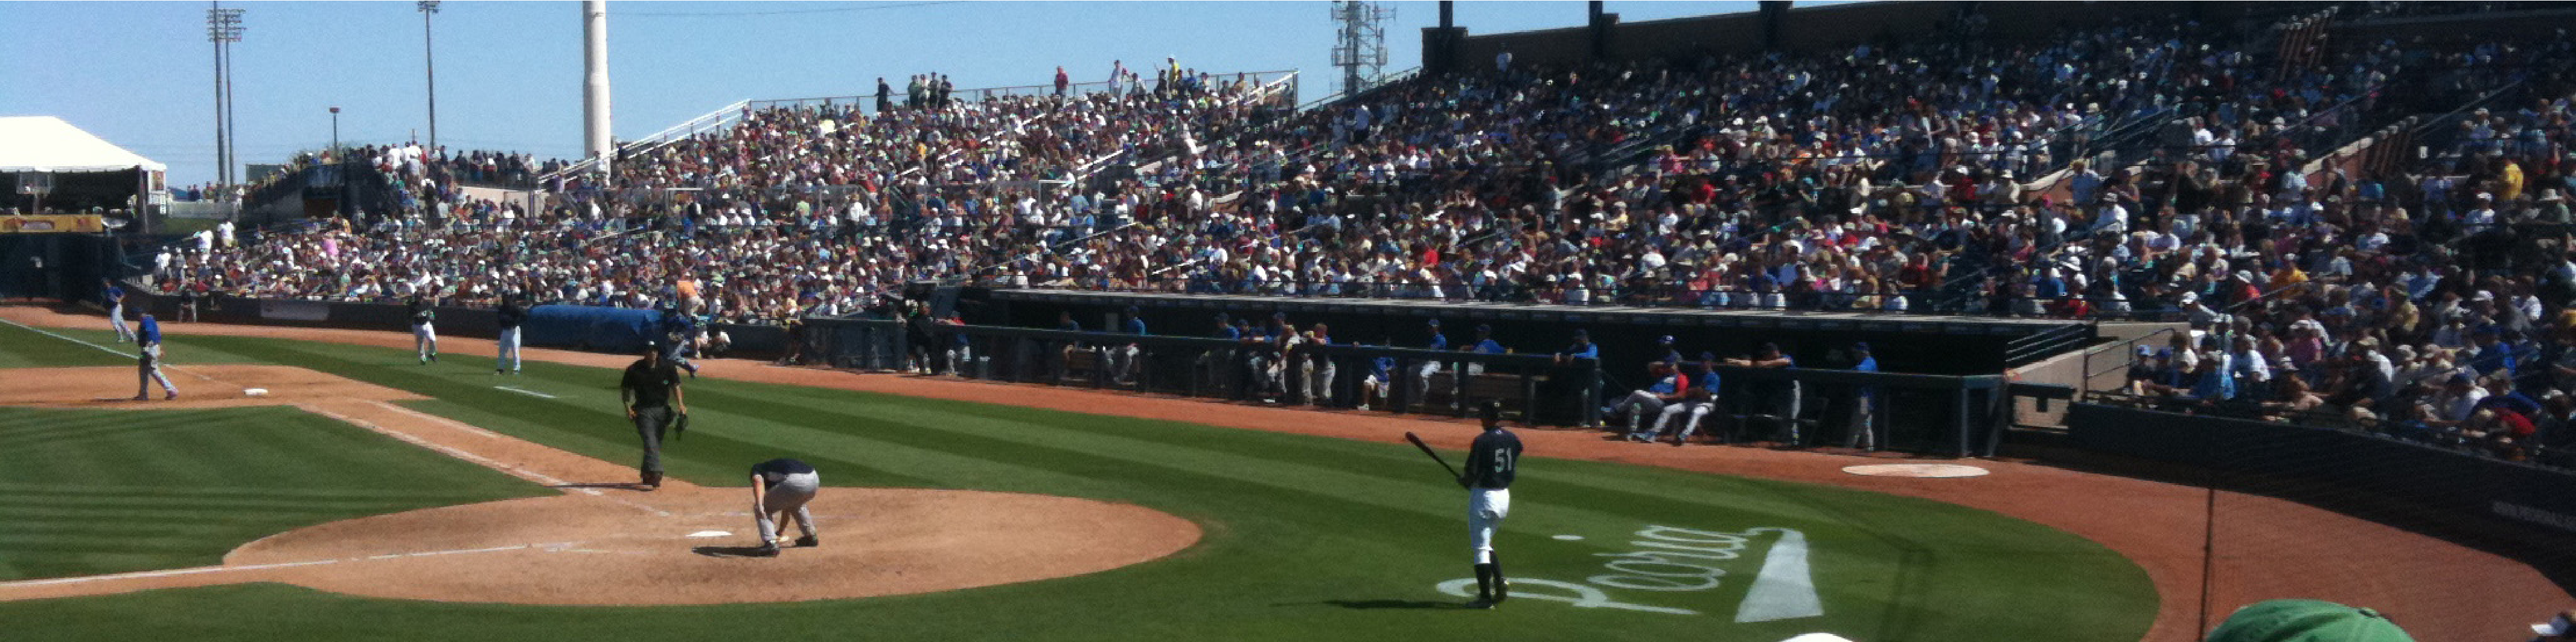
\includegraphics[width=\textwidth]{sampleteaser}
  \caption{Seattle Mariners at Spring Training, 2010.}
  \Description{Enjoying the baseball game from the third-base
  seats. Ichiro Suzuki preparing to bat.}
  \label{fig:teaser}
\end{teaserfigure}
\end{comment}
%%
%% This command processes the author and affiliation and title
%% information and builds the first part of the formatted document.

\section{Introduction}
Recently, Blockchian has become a new popular terms and area people talk about. Not only does it has tons of innovative application in technology but also the impact it impose is also huge which will overturn the world that we live in. Decentralized is the key component that catch everyone's attention. Ranging from financial technology, semiconductor industry, entertainment industry and art collection, blockchain is providing a whole new architecture of protecting and contributing the system integrity and security at the same time. The key concept that blockchain was based on decentralized consensus is like a voting system where every node participating in the network could have equal contribution to the decision of the network. \\
%% Bitcoin
Bitcoin, as the most famous cryptocurrency, has been making a huge impact to the blockchain society and the whole world. Different kind of consensus theory has been proposed ever since the launch of bitcoin. As the first truly decentralized cryptocurrency, Bitcoin launched at 2008, invented by the mistyrious anonymous founder Satoshi Nakamoto, is not only the forerunner but the motivation to any application in the blockchain expertise. \\
Etherrum, intially started with a more robust scripting language a Turing-complete programming language, was a improvement to bitcoin core algorithm. Not only does it slight tune the 21 million limitation of Bitcoin but the extension on decentralized contract system has triggered many different application accross financial technology and art exhibition. With the recent migration of the original consensus protocol, proof of work, to a more stable protocol, proof of stake, Ethereum is constantly become a better network in all aspect than its predecesor, Bitcoin. 
Proof of space is noval consensus protocol that was proposed recently since 2017. Chia network is one of network that utilize the proof of space consensus theory  \\


% \begin{figure}[ht]
% \begin{center}
% 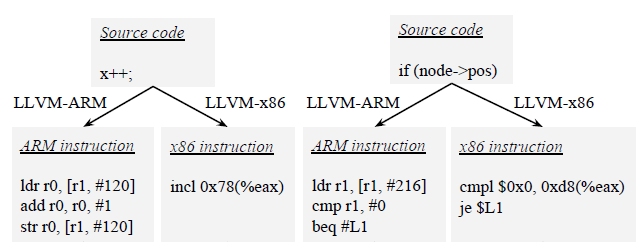
\includegraphics[height=3.75cm, width=9.5cm]{pic1.PNG}
% \end{center}
% {\footnotesize Fig. 1 ARM and x86 instructions are compiled through the same LLVM compiler. These two architecture apply totally different methods to have functionalized instructions. The discrepancies from the architectures make it difficult to validate the semantical equivalence after translation.}
% \end{figure}

\section{Chia network}
%% Chia coin
Chia was founded in May 2021 by Bram Cohen, who was known for the peer-to-peer file-sharing internet protocol, BitTorrent. The intention of building the chia decentralized network is to improve the energy consumption spend on Bitcoin mining by utilizing a new consensus, proof of space, as the fundamental of the network. \\
Chia is a decentralized consensus network that uses the combination of Proof of Space and Proof of time (VDF) as the fundamental consensus algorithm. \\
When a person owns a storage disk with 1 GB, the person can request to join the network by implementing the network protocol to claim and tell the network that he or she has a storage disk with 1 GB. How do we let the network know that you did actually hold a 1 GB storage space? In order to prove you have 1 GB space, we could simply give you a 1GB file and tell you to store the file on your disk. When we need a specific segment of information in the file, we request it from you, you should be able to pull out the exact same information. \\
In order to store the user information in the File that the network gave to the farmer and create the proof of space of earning the rewards, three stages are required in the participation of Chia network: In the following chapters, we will discuss more in detail.
Chia network is composed of three roles, timelord, farmer, and verifier. Whenever timelord releases the lottery, a sub-plot, to the network every ten minutes, farmers who have a completed plot file will construct a proof of space from the plot file they store and send the proof of space to the verifier to verify. When the verifier verifies that the exact proof of space corresponds to a sub-slot, the rewards will go to the selected farmer. The reward for successfully finding the valid proof of space is 2 XCH. Why the block generation rate is 10 mins per block\\
Three steps have to be completed before winning the rewards. \\ 
{\bf Plotting}
Plotting will store a huge amount of hash data in a plot file in order for the farmer to quickly fetch the proof of space in the next step, farming.  
Not only the hash data but the checkpoint data, which will assist in faster proof of space retrieval, will be stored in the plot file. The plotting works from table 1 through table 7. \\
{\bf Farming}
Farming is the process of consrtucting prove to the network that ones actually owns a specific amount of disk space. To begin with, the network will release a challenge to every farmer who has participating in the game. Upon receiving the challenge, farmer goes to the last table, table 7, to find the matching data along with the corresponding checkpoint, stored in plot file, subsequently traverse the search by the matching data in the previous table, table 6, and following this routine to the first table, constructing a proof of space and send it out for verifying. In reverse than plotting, farming retrive data from the last table. \\
{\bf Verifying}
The verifying stage require 
{\bf Plot filter}
The plot filter is a threshold to decide whether the challenge has any possibility of getting rewards. It is used to prevent the farmer on finding proof of space that one's doesn't have. Farmers receive these signage points and compute a hash for each plot, at each signage point. If the hash starts with nine zeros, the plot passes the filter for that signage point, and can proceed. This disqualifies around 511/512 of all plot files in the network, for that signage point. The formula to compute the filter hash is
\begin{align*}
  \text{plot filter bits} = sha256(\text{plot id} + \text{sub-slot challenge} + \text{cc signage point})
\end{align*}
{\bf Sub-slot} 
A segement of challenge that is generated by the timelord and will be issue to the farmer. The format of the sub-slot is as below
\begin{verbatim}
class ChallengeChainSubSlot(Streamable):
  challenge_chain_end_of_slot_vdf: VDFInfo
  infused_challenge_chain_sub_slot_hash: [bytes32]
  subepoch_summary_hash: [bytes32]
  new_sub_slot_iters: [uint64]
  new_difficulty: [uint64] 
\end{verbatim}
{\bf Singage Point}
The sinage point is a temporarily stage for sub-slot generating. Within 64 iteration of the sinage point, composing a complete sub-slot, each sinage point will be release by the timelord to the farmer every 9.375 seconds. The farmer, upon receiving the sinage point will compute the plot filter to see if it pass the threshold.

%% 
\section{Chia Plotting Process}
The plotting process could be analogous to the work done, such as fertilizing and irrigating then cropping the seed in the farm, while farming could be analogous to the process of harvesting the product. It begins with storing many hash-like number in a file that stores on the farmer disk. Seven tables is initiate in the plot file with a specific plot constant k. 
Two parameters will be required when plotting initialize. A plot seed, which is received from the network, a plot constant k, which is assigned by the farmer. \\
{\bf Plot constants k} The plot constants k represent the number of entries each table, which is determine by the farmer. The minumum disk space of the plot with $k = 32$ is 515.4 (GB) for temperarily storage and 104.7 (GB) for final storage. 
\begin{align*}
  \text{Number of entries in each table} = 2^{k}, 32 \leqq k \leqq 50 \\
  \text{Temporarily plot file size} \approx 3.75 \times k \times 2^{k} (byte) \\
  \text{Final plot file size } \approx 0.762 \times k \times 2^{k} (btye) \\
\end{align*}
{\bf Plot seed} The plot seed is a 32 byte constant received from the network to initialize each plot file, so that no two plot file will be the same. 
\begin{align*}
  \text{plot\_seed} \in [2^{256}] \\
\end{align*}
That is said, all the farmer need within the plotting process is the plot seed receiving online, everything else will be able to construct offline. The design of chia plotting process is intentionally design so that whomever gets a powerful machine, such as a ASIC or GPU won't create absolute advantage over those who don't, because the main motivation is letting the farmer purely use  The plotting process will be distinguish into the following four parts. \\
{\bf 1. Forward propogation}
The forward propogation is to insert data in each entries of the table, from table 1 to table 7. The dependency of the table is table i + 1 will relie on the talbe i (i = 0, 1, ... 6). Because this dependency, farmer who wish to accelerate the plotting process will not have the ability to predict what the next table content without waiting for the completion of the previous table. This will create a bottle-neck for those who wish to create a faster plotting method using a high performance machine. Other than the first stage, the rest are extra optimization feature created by Chia network. With a fully propagation plot file, the farmer are allow to construct the proof of space. But considering the efficiency, Step 2 to 3 are recommended to operating, in order to reduce unused data and make good use of the disk space\\
{\bf 2. Backward propogation}
Backward propogation is to reduce the size of each table by getting rid of those entry that's not in use. In each table, a left entry will contain data from the previous table, right entry contain data it calculate. The entry is useful to the next table, only if the left entry is equal to the right. Therefore, in this stage, it is dropping unused data where the left is not equal to the right. \\
{\bf 3. Compression}
The compression stage is to compacting the content in each table and create a format for the efficiently retrival with bucket id. The  \\
{\bf 4. Checkpoint}
Checkpoint will create a faster index for future proof retrieval. \\


{\bf Chacha8 and Blake3 hash-like function}
The fundamental of chia plot generation is based on two hash functions, chacha8 and blake3, where chacha8 is used in the gerneration of the first table and blake3 is used in generation of the rest 6 tables. The hash function will fetch in a 
{\bf Table 1}
The generation of the table 1 required iteration through the entire entries with value up to $2^{k} - 1$, which is more than 4 billion entries with k32 plot. 
\begin{figure}[ht]
\begin{center}
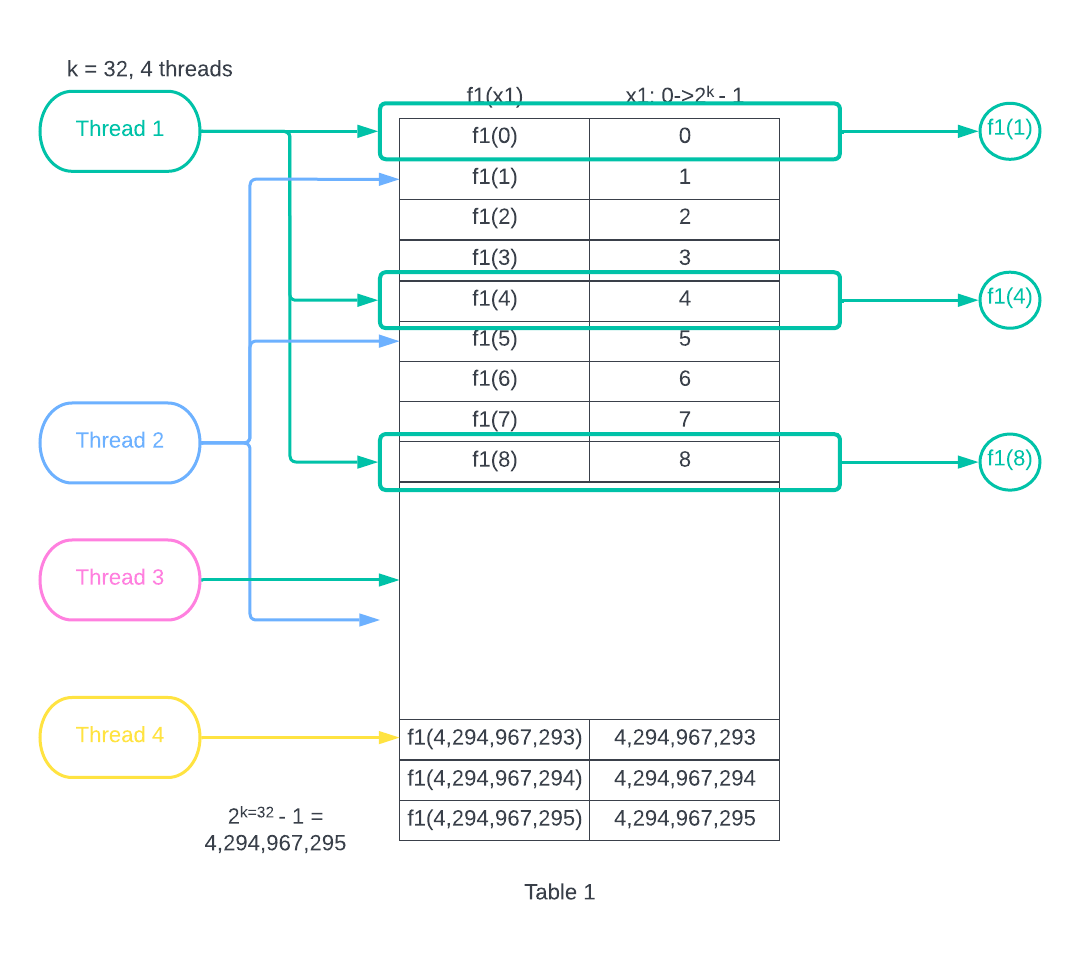
\includegraphics[height=4.5cm, width=7cm]{Speedy_Chia_Threading.png}
\end{center}
{\footnotesize Fig. 2 The generation of table 1 required at lease 4 billion iteration in a k32 plot file.}
\end{figure}

\begin{figure*}[ht]
  \begin{center}
  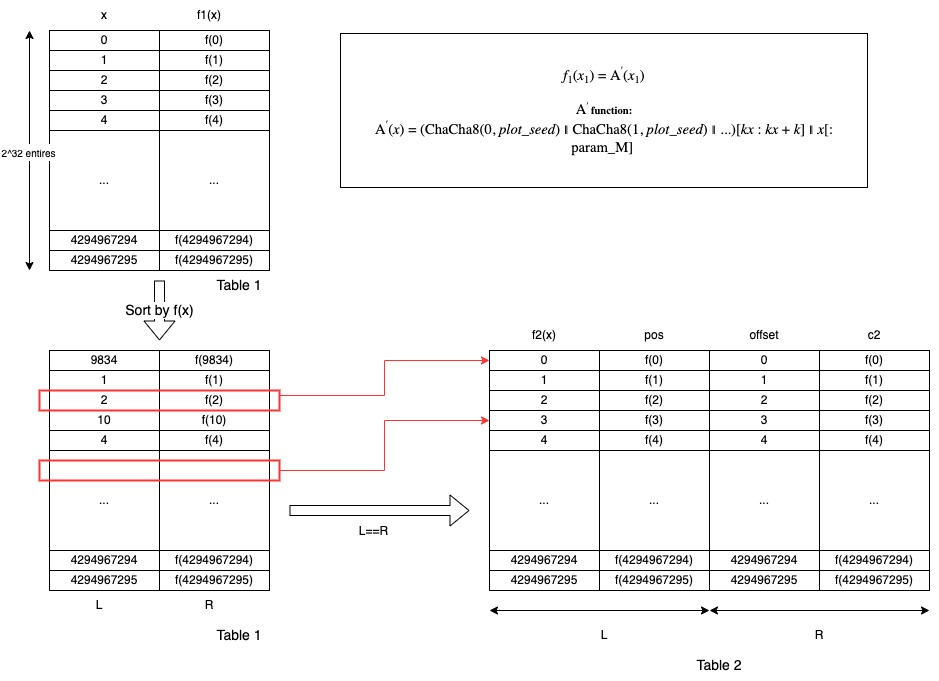
\includegraphics[height=8.5cm, width=16cm]{Chia_Plot_Process.jpeg}
  \end{center}
  {\footnotesize Fig. 3 The dependcy between table 1 and table 2.}
  \end{figure*}
{\bf Dependency between table (i) and table (i + 1)}
The dependency of table i and table i + 1 lie in that table i + 1 will required the matching entries in the left and right to calculate the offset of the tale i. 
\section{Related work}
{\bf Approach by madMax}
One of the contributors of the open-source project, XPM GPU Miner, \parencite[]{mad_chia_plotter}, has successfully provided a highly parallelize architecture to support more efficient parallel computing to accelerate chia plotting by creating multiple threads on a multi-core processor. The result of his is 17 seconds for the table 1 using a 256 GB RAM dual Xeon® E5-2650v2@2.60GHz R720 processor with 16 threads. The method he uses is to create a thread pool manager in managing the status of each thread. The thread pool manager would not benefit from the table 1 generation since all the entry calculation is done in parallel. However, the thread pool manager could benefit from the matching function in the rest of the table generation, from table 2 to table 7. When generating table 2, some thread will be doing the matching calculation, some threads will drop those that is not in use. Therefore, introducing the locking mutex in the first stage of table 2 to table 7 is necessary. In addition, madMax solution also provides a larger RAM buffer usage. Take the first stage of k32 table 1 plot file generation, the disk operation wouldn't be operating until the all entry calculation is done. About 68 (GB) of memory space will be occupied if not flushing the data to disk during table 1 plotting.
\begin{align*}
  \text{Temperarily RAM usage} &= 2^{k} |_{k = 32} (entry/table) \times 16 (bytes/entry) \\
                               &= 6.872 \times 10^{10} (Byte)
\end{align*}
\section{Approach with Parallel Computing}
% Nvidia GPU why do you think GPU could assist the plotting process
My intention of accelerating the Chia plotting starts from a post \parencite*[]{why_not_gpu_chia}, stating that it is impossible to use GPU to assist the plotting process. The reason is that using GPU to the plot will require a huge amount of temporary memory usage. If the device memory is not large enough, it will result in disk I/O operation penalties. Take k32 plot, for example, it will require more than 36 GB of memory space for storage in order to calculate table 1. The maximum device storage on an Nvidia GPU is less than 30 MB per node. Therefore, using GPU to assist the plotting, we still have to store the temporary plot file somewhere before writing back to disk space. 
% Address the memory limitation device memory: 32 MB
\begin{figure}[ht]
  \begin{center}
  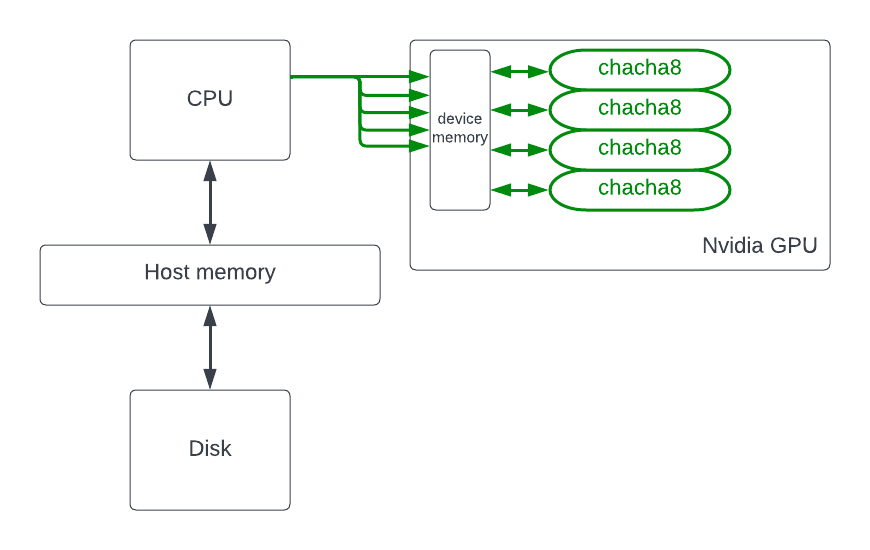
\includegraphics[height=4.5cm, width=7cm]{Chia_GPU_architecture.png}
  \end{center}
  {\footnotesize Fig. 4 The architecture of GPU accelerated computing Chia plot.}
  \end{figure}
{\bf Software architecture}
Adding the threading queue in front of GPU kernel function. Memory copying from host to device side is costly, and the approach is to copy data together to the kernel device at once to reduce the cost of issuing memory copy seperatly. The queue will collect data derived and iterated from the table 1 function and issue to the kernel when the queue is collecting enough data for GPU to calculate at the same working cycle. 

% synchronize issue among different thread
Regarding the synchronize issue among all different thread, no mutex is requird for the generation of the 1st table. Since each entry is independent to each other, so the writing to disk would be affected by the lock mechanism.  
\section{Result - without GPU}
The implementation of mine is based on the calculation of the table 1. The generation of table 1 will require the chacha8 hash function which could be done in parallel. The result running on the TAMU Grace super computer cluster is approximately 900 seconds for k32 plot file and 1833 seconds for k33 plot file. The temporarily storage in k32 plot file is around 36 GB. While k33 plot file is around 76 GB. 
\begin{table}
  \caption{Frequency of Special Characters}
  \label{tab:freq}
  \begin{tabular}{ccccl}
    \toprule
    Plot constant k&Thread number&Time (sec)&Average (sec)\\
    \midrule
      & 4   & 911.52 &       \\
    32& 8   & 908.96 & 908.23\\
      & 16  & 906.99 &       \\
      & 32  & 905.46 &       \\
  \bottomrule
      & 4   & 1840.32 &         \\
    33& 8   & 1840.91 & 1833.53 \\
      & 16  & 1825.87 &         \\
      & 32  & 1827.00 &         \\
\bottomrule
\end{tabular}
\end{table}


\section{Conclusions}
After evaluating the enhancements and implementation difficulties, I proposed my view of possible solutions to this topic. Using super-computer clusters with accelerated units or with a larger memory space will effectively improve the plotting speed in different aspects, however, the hardware cost is also one aspect everyone dedicating to using this solution has to take into serious consideration.  \\
Conclusively, the result shows positive outcomes with respect to using the official source code on a simple desktop machine. Although future optimization is required to perfect the solution, I could conclude that the survey has left with some positive consequences.
\parencite{chia_github} \parencite*[]{chia_github_doc} 
\parencite{2_vdf}
\section{Future Work}
The future work will be focusing on improving the threading algorithm and the memory cache issue, with specifically what to keep in the temporarily storage and what not to keep in the temporarily storage. \\
{\bf RAM usage} 
Memory usage has been very cautious, my intention is not to overuse the memory space at the first attempt, therefore, my approach will still be limited by the disk I/O latency whenever writing 256 buckets of entry data from memory to disk during plotting frequently. But as discussed in the madMax solution, caching more data in memory before writing to disk will eliminate a huge amount of time. Therefore, the first optimization I will do regarding the current development is to cache more entries in memory and to write more buckets out to disk at the same event. \\
{\bf Thread Pool}
A threading pool manager will be added in order to handle the completion of each thread. The existence of the thread pool manager is to assist the rest of the tables when some of the threads might be doing one thing differently from the other. In addition to the entry calculation in table 2, the matching function search through table 1 will also be one of the tasks that could be done in parallel along with the entry calculation. 
\section{Reference}
\printbibliography[heading=none]

\begin{comment}
\section{Introduction}
ACM's consolidated article template, introduced in 2017, provides a
consistent \LaTeX\ style for use across ACM publications, and
incorporates accessibility and metadata-extraction functionality
necessary for future Digital Library endeavors. Numerous ACM and
SIG-specific \LaTeX\ templates have been examined, and their unique
features incorporated into this single new template.

If you are new to publishing with ACM, this document is a valuable
guide to the process of preparing your work for publication. If you
have published with ACM before, this document provides insight and
instruction into more recent changes to the article template.

The ``\verb|acmart|'' document class can be used to prepare articles
for any ACM publication --- conference or journal, and for any stage
of publication, from review to final ``camera-ready'' copy, to the
author's own version, with {\itshape very} few changes to the source.

\section{Template Overview}
As noted in the introduction, the ``\verb|acmart|'' document class can
be used to prepare many different kinds of documentation --- a
double-blind initial submission of a full-length technical paper, a
two-page SIGGRAPH Emerging Technologies abstract, a ``camera-ready''
journal article, a SIGCHI Extended Abstract, and more --- all by
selecting the appropriate {\itshape template style} and {\itshape
  template parameters}.

This document will explain the major features of the document
class. For further information, the {\itshape \LaTeX\ User's Guide} is
available from
\url{https://www.acm.org/publications/proceedings-template}.

\subsection{Template Styles}

The primary parameter given to the ``\verb|acmart|'' document class is
the {\itshape template style} which corresponds to the kind of publication
or SIG publishing the work. This parameter is enclosed in square
brackets and is a part of the {\verb|documentclass|} command:
\begin{verbatim}
  \documentclass[STYLE]{acmart}
\end{verbatim}

Journals use one of three template styles. All but three ACM journals
use the {\verb|acmsmall|} template style:
\begin{itemize}
\item {\verb|acmsmall|}: The default journal template style.
\item {\verb|acmlarge|}: Used by JOCCH and TAP.
\item {\verb|acmtog|}: Used by TOG.
\end{itemize}

The majority of conference proceedings documentation will use the {\verb|acmconf|} template style.
\begin{itemize}
\item {\verb|acmconf|}: The default proceedings template style.
\item{\verb|sigchi|}: Used for SIGCHI conference articles.
\item{\verb|sigchi-a|}: Used for SIGCHI ``Extended Abstract'' articles.
\item{\verb|sigplan|}: Used for SIGPLAN conference articles.
\end{itemize}

\subsection{Template Parameters}

In addition to specifying the {\itshape template style} to be used in
formatting your work, there are a number of {\itshape template parameters}
which modify some part of the applied template style. A complete list
of these parameters can be found in the {\itshape \LaTeX\ User's Guide.}

Frequently-used parameters, or combinations of parameters, include:
\begin{itemize}
\item {\verb|anonymous,review|}: Suitable for a ``double-blind''
  conference submission. Anonymizes the work and includes line
  numbers. Use with the \verb|\acmSubmissionID| command to print the
  submission's unique ID on each page of the work.
\item{\verb|authorversion|}: Produces a version of the work suitable
  for posting by the author.
\item{\verb|screen|}: Produces colored hyperlinks.
\end{itemize}

This document uses the following string as the first command in the
source file:
\begin{verbatim}
\documentclass[sigplan,screen]{acmart}
\end{verbatim}

\section{Modifications}

Modifying the template --- including but not limited to: adjusting
margins, typeface sizes, line spacing, paragraph and list definitions,
and the use of the \verb|\vspace| command to manually adjust the
vertical spacing between elements of your work --- is not allowed.

{\bfseries Your document will be returned to you for revision if
  modifications are discovered.}

\section{Typefaces}

The ``\verb|acmart|'' document class requires the use of the
``Libertine'' typeface family. Your \TeX\ installation should include
this set of packages. Please do not substitute other typefaces. The
``\verb|lmodern|'' and ``\verb|ltimes|'' packages should not be used,
as they will override the built-in typeface families.

\section{Title Information}

The title of your work should use capital letters appropriately -
\url{https://capitalizemytitle.com/} has useful rules for
capitalization. Use the {\verb|title|} command to define the title of
your work. If your work has a subtitle, define it with the
{\verb|subtitle|} command.  Do not insert line breaks in your title.

If your title is lengthy, you must define a short version to be used
in the page headers, to prevent overlapping text. The \verb|title|
command has a ``short title'' parameter:
\begin{verbatim}
  \title[short title]{full title}
\end{verbatim}

\section{Authors and Affiliations}

Each author must be defined separately for accurate metadata
identification. Multiple authors may share one affiliation. Authors'
names should not be abbreviated; use full first names wherever
possible. Include authors' e-mail addresses whenever possible.

Grouping authors' names or e-mail addresses, or providing an ``e-mail
alias,'' as shown below, is not acceptable:
\begin{verbatim}
  \author{Brooke Aster, David Mehldau}
  \email{dave,judy,steve@university.edu}
  \email{firstname.lastname@phillips.org}
\end{verbatim}

The \verb|authornote| and \verb|authornotemark| commands allow a note
to apply to multiple authors --- for example, if the first two authors
of an article contributed equally to the work.

If your author list is lengthy, you must define a shortened version of
the list of authors to be used in the page headers, to prevent
overlapping text. The following command should be placed just after
the last \verb|\author{}| definition:
\begin{verbatim}
  \renewcommand{\shortauthors}{McCartney, et al.}
\end{verbatim}
Omitting this command will force the use of a concatenated list of all
of the authors' names, which may result in overlapping text in the
page headers.

The article template's documentation, available at
\url{https://www.acm.org/publications/proceedings-template}, has a
complete explanation of these commands and tips for their effective
use.

Note that authors' addresses are mandatory for journal articles.

\section{Rights Information}

Authors of any work published by ACM will need to complete a rights
form. Depending on the kind of work, and the rights management choice
made by the author, this may be copyright transfer, permission,
license, or an OA (open access) agreement.

Regardless of the rights management choice, the author will receive a
copy of the completed rights form once it has been submitted. This
form contains \LaTeX\ commands that must be copied into the source
document. When the document source is compiled, these commands and
their parameters add formatted text to several areas of the final
document:
\begin{itemize}
\item the ``ACM Reference Format'' text on the first page.
\item the ``rights management'' text on the first page.
\item the conference information in the page header(s).
\end{itemize}

Rights information is unique to the work; if you are preparing several
works for an event, make sure to use the correct set of commands with
each of the works.

The ACM Reference Format text is required for all articles over one
page in length, and is optional for one-page articles (abstracts).

\section{CCS Concepts and User-Defined Keywords}

Two elements of the ``acmart'' document class provide powerful
taxonomic tools for you to help readers find your work in an online
search.

The ACM Computing Classification System ---
\url{https://www.acm.org/publications/class-2012} --- is a set of
classifiers and concepts that describe the computing
discipline. Authors can select entries from this classification
system, via \url{https://dl.acm.org/ccs/ccs.cfm}, and generate the
commands to be included in the \LaTeX\ source.

User-defined keywords are a comma-separated list of words and phrases
of the authors' choosing, providing a more flexible way of describing
the research being presented.

CCS concepts and user-defined keywords are required for for all
articles over two pages in length, and are optional for one- and
two-page articles (or abstracts).

\section{Sectioning Commands}

Your work should use standard \LaTeX\ sectioning commands:
\verb|section|, \verb|subsection|, \verb|subsubsection|, and
\verb|paragraph|. They should be numbered; do not remove the numbering
from the commands.

Simulating a sectioning command by setting the first word or words of
a paragraph in boldface or italicized text is {\bfseries not allowed.}

\section{Tables}

The ``\verb|acmart|'' document class includes the ``\verb|booktabs|''
package --- \url{https://ctan.org/pkg/booktabs} --- for preparing
high-quality tables.

Table captions are placed {\itshape above} the table.

Because tables cannot be split across pages, the best placement for
them is typically the top of the page nearest their initial cite.  To
ensure this proper ``floating'' placement of tables, use the
environment \textbf{table} to enclose the table's contents and the
table caption.  The contents of the table itself must go in the
\textbf{tabular} environment, to be aligned properly in rows and
columns, with the desired horizontal and vertical rules.  Again,
detailed instructions on \textbf{tabular} material are found in the
\textit{\LaTeX\ User's Guide}.

Immediately following this sentence is the point at which
Table~\ref{tab:freq} is included in the input file; compare the
placement of the table here with the table in the printed output of
this document.

\begin{table}
  \caption{Frequency of Special Characters}
  \label{tab:freq}
  \begin{tabular}{ccl}
    \toprule
    Non-English or Math&Frequency&Comments\\
    \midrule
    \O & 1 in 1,000& For Swedish names\\
    $\pi$ & 1 in 5& Common in math\\
    \$ & 4 in 5 & Used in business\\
    $\Psi^2_1$ & 1 in 40,000& Unexplained usage\\
  \bottomrule
\end{tabular}
\end{table}

To set a wider table, which takes up the whole width of the page's
live area, use the environment \textbf{table*} to enclose the table's
contents and the table caption.  As with a single-column table, this
wide table will ``float'' to a location deemed more
desirable. Immediately following this sentence is the point at which
Table~\ref{tab:commands} is included in the input file; again, it is
instructive to compare the placement of the table here with the table
in the printed output of this document.

\begin{table*}
  \caption{Some Typical Commands}
  \label{tab:commands}
  \begin{tabular}{ccl}
    \toprule
    Command &A Number & Comments\\
    \midrule
    \texttt{{\char'134}author} & 100& Author \\
    \texttt{{\char'134}table}& 300 & For tables\\
    \texttt{{\char'134}table*}& 400& For wider tables\\
    \bottomrule
  \end{tabular}
\end{table*}

Always use midrule to separate table header rows from data rows, and
use it only for this purpose. This enables assistive technologies to
recognise table headers and support their users in navigating tables
more easily.

\section{Math Equations}
You may want to display math equations in three distinct styles:
inline, numbered or non-numbered display.  Each of the three are
discussed in the next sections.

\subsection{Inline (In-text) Equations}
A formula that appears in the running text is called an inline or
in-text formula.  It is produced by the \textbf{math} environment,
which can be invoked with the usual
\texttt{{\char'134}begin\,\ldots{\char'134}end} construction or with
the short form \texttt{\$\,\ldots\$}. You can use any of the symbols
and structures, from $\alpha$ to $\omega$, available in
\LaTeX~\cite{Lamport:LaTeX}; this section will simply show a few
examples of in-text equations in context. Notice how this equation:
\begin{math}
  \lim_{n\rightarrow \infty}x=0
\end{math},
set here in in-line math style, looks slightly different when
set in display style.  (See next section).

\subsection{Display Equations}
A numbered display equation---one set off by vertical space from the
text and centered horizontally---is produced by the \textbf{equation}
environment. An unnumbered display equation is produced by the
\textbf{displaymath} environment.

Again, in either environment, you can use any of the symbols and
structures available in \LaTeX\@; this section will just give a couple
of examples of display equations in context.  First, consider the
equation, shown as an inline equation above:
\begin{equation}
  \lim_{n\rightarrow \infty}x=0
\end{equation}
Notice how it is formatted somewhat differently in
the \textbf{displaymath}
environment.  Now, we'll enter an unnumbered equation:
\begin{displaymath}
  \sum_{i=0}^{\infty} x + 1
\end{displaymath}
and follow it with another numbered equation:
\begin{equation}
  \sum_{i=0}^{\infty}x_i=\int_{0}^{\pi+2} f
\end{equation}
just to demonstrate \LaTeX's able handling of numbering.

\section{Figures}

The ``\verb|figure|'' environment should be used for figures. One or
more images can be placed within a figure. If your figure contains
third-party material, you must clearly identify it as such, as shown
in the example below.
\begin{figure}[h]
  \centering
  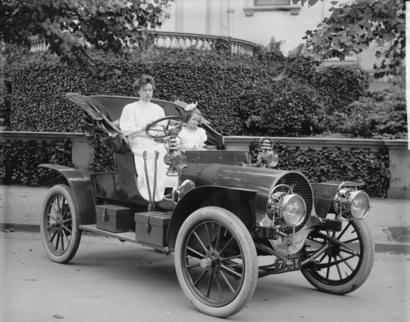
\includegraphics[width=\linewidth]{sample-franklin}
  \caption{1907 Franklin Model D roadster. Photograph by Harris \&
    Ewing, Inc. [Public domain], via Wikimedia
    Commons. (\url{https://goo.gl/VLCRBB}).}
  \Description{A woman and a girl in white dresses sit in an open car.}
\end{figure}

Your figures should contain a caption which describes the figure to
the reader.

Figure captions are placed {\itshape below} the figure.

Every figure should also have a figure description unless it is purely
decorative. These descriptions convey what’s in the image to someone
who cannot see it. They are also used by search engine crawlers for
indexing images, and when images cannot be loaded.

A figure description must be unformatted plain text less than 2000
characters long (including spaces).  {\bfseries Figure descriptions
  should not repeat the figure caption – their purpose is to capture
  important information that is not already provided in the caption or
  the main text of the paper.} For figures that convey important and
complex new information, a short text description may not be
adequate. More complex alternative descriptions can be placed in an
appendix and referenced in a short figure description. For example,
provide a data table capturing the information in a bar chart, or a
structured list representing a graph.  For additional information
regarding how best to write figure descriptions and why doing this is
so important, please see
\url{https://www.acm.org/publications/taps/describing-figures/}.

\subsection{The ``Teaser Figure''}

A ``teaser figure'' is an image, or set of images in one figure, that
are placed after all author and affiliation information, and before
the body of the article, spanning the page. If you wish to have such a
figure in your article, place the command immediately before the
\verb|\maketitle| command:
\begin{verbatim}
  \begin{teaserfigure}
    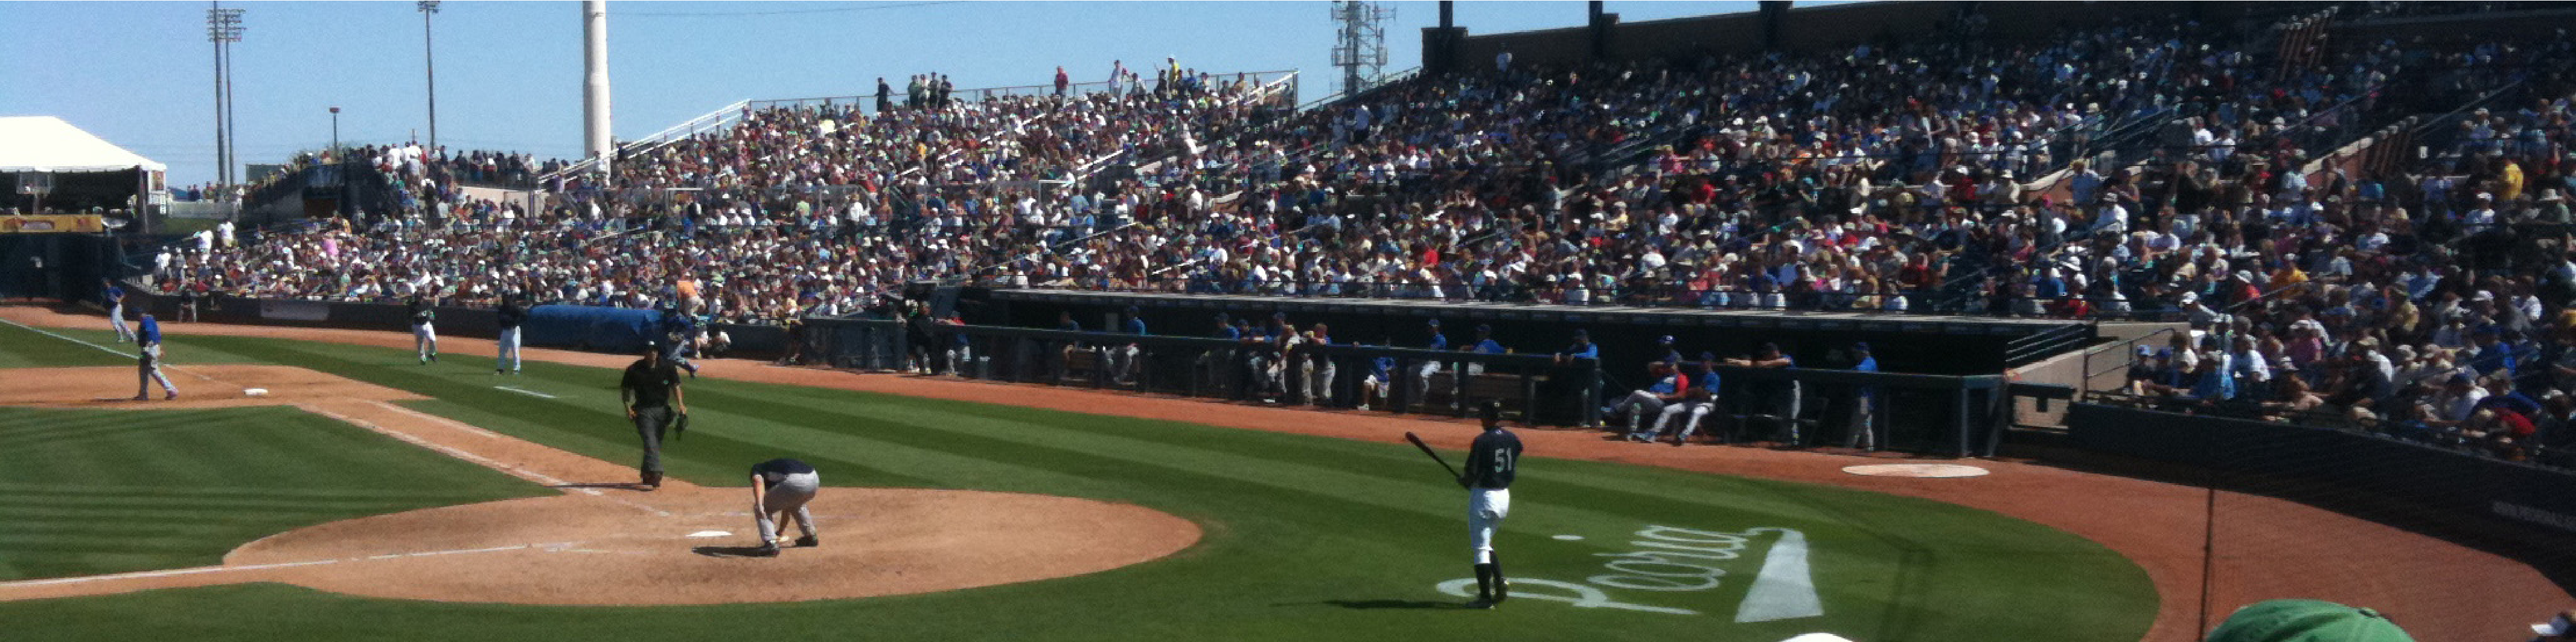
\includegraphics[width=\textwidth]{sampleteaser}
    \caption{figure caption}
    \Description{figure description}
  \end{teaserfigure}
\end{verbatim}

\section{Citations and Bibliographies}

The use of \BibTeX\ for the preparation and formatting of one's
references is strongly recommended. Authors' names should be complete
--- use full first names (``Donald E. Knuth'') not initials
(``D. E. Knuth'') --- and the salient identifying features of a
reference should be included: title, year, volume, number, pages,
article DOI, etc.

The bibliography is included in your source document with these two
commands, placed just before the \verb|\end{document}| command:
\begin{verbatim}
  \bibliographystyle{ACM-Reference-Format}
  \bibliography{bibfile}
\end{verbatim}
where ``\verb|bibfile|'' is the name, without the ``\verb|.bib|''
suffix, of the \BibTeX\ file.

Citations and references are numbered by default. A small number of
ACM publications have citations and references formatted in the
``author year'' style; for these exceptions, please include this
command in the {\bfseries preamble} (before the command
``\verb|\begin{document}|'') of your \LaTeX\ source:
\begin{verbatim}
  \citestyle{acmauthoryear}
\end{verbatim}

  Some examples.  A paginated journal article \cite{Abril07}, an
  enumerated journal article \cite{Cohen07}, a reference to an entire
  issue \cite{JCohen96}, a monograph (whole book) \cite{Kosiur01}, a
  monograph/whole book in a series (see 2a in spec. document)
  \cite{Harel79}, a divisible-book such as an anthology or compilation
  \cite{Editor00} followed by the same example, however we only output
  the series if the volume number is given \cite{Editor00a} (so
  Editor00a's series should NOT be present since it has no vol. no.),
  a chapter in a divisible book \cite{Spector90}, a chapter in a
  divisible book in a series \cite{Douglass98}, a multi-volume work as
  book \cite{Knuth97}, a couple of articles in a proceedings (of a
  conference, symposium, workshop for example) (paginated proceedings
  article) \cite{Andler79, Hagerup1993}, a proceedings article with
  all possible elements \cite{Smith10}, an example of an enumerated
  proceedings article \cite{VanGundy07}, an informally published work
  \cite{Harel78}, a couple of preprints \cite{Bornmann2019,
    AnzarootPBM14}, a doctoral dissertation \cite{Clarkson85}, a
  master's thesis: \cite{anisi03}, an online document / world wide web
  resource \cite{Thornburg01, Ablamowicz07, Poker06}, a video game
  (Case 1) \cite{Obama08} and (Case 2) \cite{Novak03} and \cite{Lee05}
  and (Case 3) a patent \cite{JoeScientist001}, work accepted for
  publication \cite{rous08}, 'YYYYb'-test for prolific author
  \cite{SaeediMEJ10} and \cite{SaeediJETC10}. Other cites might
  contain 'duplicate' DOI and URLs (some SIAM articles)
  \cite{Kirschmer:2010:AEI:1958016.1958018}. Boris / Barbara Beeton:
  multi-volume works as books \cite{MR781536} and \cite{MR781537}. A
  couple of citations with DOIs:
  \cite{2004:ITE:1009386.1010128,Kirschmer:2010:AEI:1958016.1958018}. Online
  citations: \cite{TUGInstmem, Thornburg01, CTANacmart}. Artifacts:
  \cite{R} and \cite{UMassCitations}.

\section{Acknowledgments}

Identification of funding sources and other support, and thanks to
individuals and groups that assisted in the research and the
preparation of the work should be included in an acknowledgment
section, which is placed just before the reference section in your
document.

This section has a special environment:
\begin{verbatim}
  \begin{acks}
  ...
  \end{acks}
\end{verbatim}
so that the information contained therein can be more easily collected
during the article metadata extraction phase, and to ensure
consistency in the spelling of the section heading.

Authors should not prepare this section as a numbered or unnumbered {\verb|\section|}; please use the ``{\verb|acks|}'' environment.

\section{Appendices}

If your work needs an appendix, add it before the
``\verb|\end{document}|'' command at the conclusion of your source
document.

Start the appendix with the ``\verb|appendix|'' command:
\begin{verbatim}
  \appendix
\end{verbatim}
and note that in the appendix, sections are lettered, not
numbered. This document has two appendices, demonstrating the section
and subsection identification method.

\section{SIGCHI Extended Abstracts}

The ``\verb|sigchi-a|'' template style (available only in \LaTeX\ and
not in Word) produces a landscape-orientation formatted article, with
a wide left margin. Three environments are available for use with the
``\verb|sigchi-a|'' template style, and produce formatted output in
the margin:
\begin{itemize}
\item {\verb|sidebar|}:  Place formatted text in the margin.
\item {\verb|marginfigure|}: Place a figure in the margin.
\item {\verb|margintable|}: Place a table in the margin.
\end{itemize}

%%
%% The acknowledgments section is defined using the "acks" environment
%% (and NOT an unnumbered section). This ensures the proper
%% identification of the section in the article metadata, and the
%% consistent spelling of the heading.
\begin{acks}
To Robert, for the bagels and explaining CMYK and color spaces.
\end{acks}

%%
%% The next two lines define the bibliography style to be used, and
%% the bibliography file.
\bibliographystyle{ACM-Reference-Format}
\bibliography{sample-base}

%%
%% If your work has an appendix, this is the place to put it.
\appendix

\section{Research Methods}

\subsection{Part One}

Lorem ipsum dolor sit amet, consectetur adipiscing elit. Morbi
malesuada, quam in pulvinar varius, metus nunc fermentum urna, id
sollicitudin purus odio sit amet enim. Aliquam ullamcorper eu ipsum
vel mollis. Curabitur quis dictum nisl. Phasellus vel semper risus, et
lacinia dolor. Integer ultricies commodo sem nec semper.

\subsection{Part Two}

Etiam commodo feugiat nisl pulvinar pellentesque. Etiam auctor sodales
ligula, non varius nibh pulvinar semper. Suspendisse nec lectus non
ipsum convallis congue hendrerit vitae sapien. Donec at laoreet
eros. Vivamus non purus placerat, scelerisque diam eu, cursus
ante. Etiam aliquam tortor auctor efficitur mattis.

\section{Online Resources}

Nam id fermentum dui. Suspendisse sagittis tortor a nulla mollis, in
pulvinar ex pretium. Sed interdum orci quis metus euismod, et sagittis
enim maximus. Vestibulum gravida massa ut felis suscipit
congue. Quisque mattis elit a risus ultrices commodo venenatis eget
dui. Etiam sagittis eleifend elementum.

Nam interdum magna at lectus dignissim, ac dignissim lorem
rhoncus. Maecenas eu arcu ac neque placerat aliquam. Nunc pulvinar
massa et mattis lacinia.
\end{comment}
\end{document}
\endinput
%%
%% End of file `sample-sigplan.tex'.
